\chapter{大規模脳ネットワークの力学：トリプルネットワーク・モデル}

20世紀末からの安静時機能的磁気共鳴画像法（rs-fMRI）の進展は、脳科学に「機能局在論」から「大規模機能的結合ネットワーク（Large-Scale Brain Networks）」へのパラダイムシフトをもたらした。脳は孤立した機能野の集合ではなく、遠隔に分散する領域群が同期振動する動的システムとして作動する。
その中核を担うのが、以下の3大ネットワークである。

\begin{itemize}
  \item \textbf{DMN（デフォルト・モード・ネットワーク / Default Mode Network）}：\\
  安静時・内省時に同期し、タスク遂行時に活動が減弱（タスク負相関）する領域群（mPFC, PCC, IPLなど）。自己参照的思考、エピソード記憶の想起、未来シミュレーション、および自己物語（ナラティブ）の構築を司る。
  \item \textbf{CEN（中央実行系ネットワーク / Central Executive Network）}：\\
  背外側前頭前皮質（dlPFC）および後頭頂皮質（PPC）を中心とし、ワーキングメモリ、論理的推論、問題解決など、外部タスクに対する能動的・意識的な計算処理を実行する。
  \item \textbf{SN（顕著性ネットワーク / Salience Network）}：\\
  島皮質前部（AI）および背側前帯状皮質（dACC）を中心とし、体内外の刺激から生存や目標にとっての「顕著性（salience）」を検知し、全脳の計算リソース配分を切り替える。
\end{itemize}

\section{DMNの計算論的本質：自己防衛とナラティブ生成}
\label{section:DMNの働き}

DMNの本質は、生体内部の自己保全・ホメオスタシス維持を目的とした「自己防衛モジュール」である。その主要な計算処理は次の4点に集約される。

\begin{enumerate}[label=(\arabic*)]
  \item \textbf{刺激の自己関連付け評価}：外界からの入力を、自我（Ego）に対する「利益（profit）」「中立（neutral）」「脅威（threat）」へ即座に分類する。
  \item \textbf{自己物語（ナラティブ）の編纂}：刺激の性質に基づき、Egoを主役に据えた文脈・ストーリーを生成する。集団内の社会的ヒエラルキーや相対的ポジションの監視もここに含まれる。
  \item \textbf{因果仮説の探索}：入力刺激および生じた情動出力に対し、納得し得る因果関係を過去の記憶から逆引きする。
  \item \textbf{未来の予測と更新}：不完全な情報環境下であっても、Ego中心のモデルに基づいて未来の不確実性を先回りしてシミュレーションし続ける。
\end{enumerate}

DMNは神経系の擬似ベイズ推論器として機能し、暫定的なナラティブ仮説が確定するまで環境および記憶から貪欲にサンプリングを行う。この際、計算資源の節約と不確実性の早期解消（エントロピー低減）を最優先するため、厳密な客観的事実よりも「直感的に辻褄が合う短絡的な仮説」が優先採択されやすい。
こうして「脅威」と確定された予測は、扁桃体を中心とする大脳辺縁系を急激に励起させ、上位プロセスへの情動的割り込み（インターラプション）によって闘争・逃走反応を強制起動する。

\section{トリプルネットワーク・モデルとSNの動的スイッチング}

ヴィノッド・メノン（Vinod Menon）とルシン・ウディン（Lucina Uddin）らは、因果結合性解析（Granger因果性、動的因果モデリング）を通じて「トリプルネットワーク・モデル」を確立した。
外部課題を担うCENと、内省・反芻を担うDMNは、一方が活性化すると他方が抑制される排他・反相関関係（シーソー効果）にある。SN（特に右島皮質前部：rAI）はこのシーソーの傾きを決定づける\textbf{「因果的司令塔（Causal Outflow Hub）」}として振る舞う。

\begin{figure}[htbp]
  \centering
  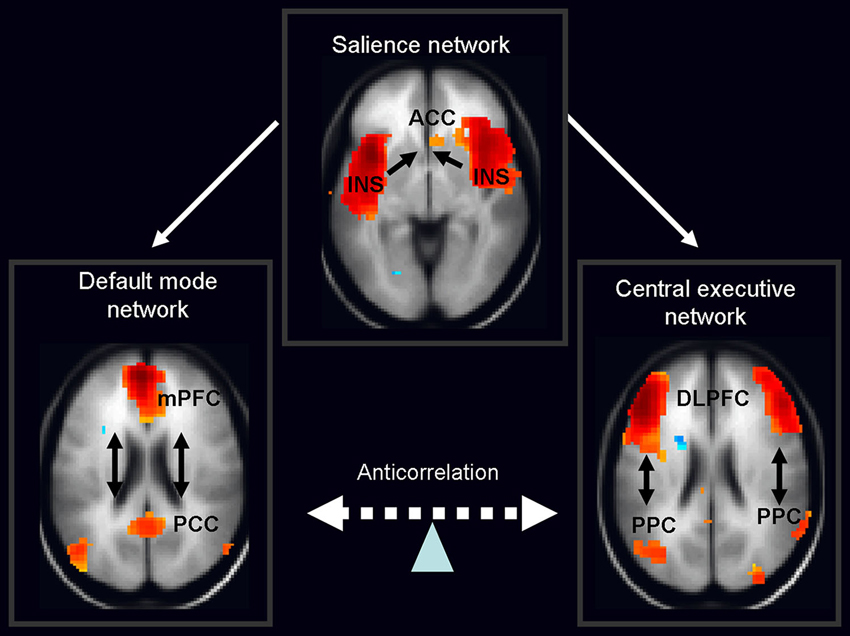
\includegraphics[width=0.82\linewidth]{src/images/triple_network_seesaw.jpg}
  \caption{Triple Network Architecture and Anticorrelated Dynamics. 
           The Salience Network (SN) dynamically modulates the seesaw equilibrium between 
           the Default Mode Network (DMN) and the Central Executive Network (CEN), 
           serving as the empirical neurobiological basis for the discrete states 
           $\mthState' = \mthState{DMN}$ and $\mthState' = \mthState{CEN}$. 
           \newline
           {\footnotesize \textbf{Credit:} By Nekovarova, Fajnerova, Horacek, Spaniel -- 
           \emph{Bridging disparate symptoms of schizophrenia: a triple network dysfunction theory}, 
           licensed under CC BY 3.0 (via Wikimedia Commons).}}
  \label{fig:triple-network-seesaw}
\end{figure}


被験者が「将来への不安や後悔」といった自己言及的ループ（DMN優位状態）に拘束されているとき、PCCやmPFCの代謝シグナルは極大化する。しかし、被験者が呼吸に伴う触覚や接地圧といった\textbf{直接的な内受容感覚（Interoception）へ急峻に注意を固定}した瞬間、以下の動態が連鎖する。

\begin{enumerate}[label=(\arabic*)]
  \item \textbf{SNのバースト同期}：島皮質前部（AI）および背側前帯状皮質（dACC）が内受容シグナルを検知し、急激に賦活化する。
  \item \textbf{DMNへの下向抑制}：活性化したSNから強力な抑制性シグナルが出力され、暴走していたDMN（PCC/mPFC）の活動が基底レベルまで強制減衰する。
  \item \textbf{計算リソースの再配分}：自己参照的なナラティブ生成が物理的に遮断され、外受容・作業記憶を司るCEN、あるいは一次感覚野へと実行帯域が再割り当てされる。
\end{enumerate}

すなわち、雑念や不安というDMNの暴走は、意志の力ではなく、SNに対する「直接的身体入力」という物理トリガーによって決定論的に鎮静化できる。
